\chapter{Tools for the LHC}
\label{ch:LHCtools}
Including data from a wide range of LHC or collider sources into a global PDF determination provides several challenges, particularly in the context of the computationally intensive 
NNPDF methodology. In this chapter we shall discuss some of the methods that have been developed in order to study the impact of collider data, and include their constraints into
PDF fits.

Firstly we shall describe the method of Bayesian reweighting of Monte Carlo error sets, along with the associated set of tools made available by a Bayesian study of PDF sets and their uncertainties.
Secondly the FastKernel method developed by the NNPDF collaboration for the fast evolution of PDFs will be introduced, along with its extension to the fast computation of experimental observables in the {\tt FK} method.
Finally we shall discuss the application of interpolation methods such as FastKernel to the automated calculation of cross sections at next-to-leading order accuracy in QCD. To this end
we shall perform a brief overview of such calculations in the context of general purpose event generators.

\section{Bayesian reweighting}
When examining the statistical properties of PDF fits it is important to note that in the Monte Carlo approach, not only the uncertainties on PDFs are provided, but a full representation of the probability distribution.
As described in Section~\ref{sec:errors}, the integral over the PDF probability distribution is approximated by a sum over replicas,
\ba \left<f\right>(x,Q^2) &=& \int f(x,Q^2) \mathcal{P}\left(f \middle| d\right) \mathcal{D}f \nonumber \\
&\approx& \frac{1}{N_{\text{rep}}}\sum_i^{N_{\text{rep}}}f_i(x,Q^2),
\ea
where the subscript $i$ here refers to the PDF replica in the Monte Carlo ensemble. This correspondence leaves PDFs in the Monte Carlo representation open to standard statistical analysis methods. One of the most important of which is the \emph{Bayesian reweighting} technique, first proposed by Giele and Keller
alongside the original Monte Carlo procedure~\cite{Giele:1998gw} and then subsequently developed by the NNPDF collaboration~\cite{Ball:2011gg,Ball:2010gb}. The problem that reweighting seeks to address is the rapid addition of experimental data into an existing parton determination. The method is particularly useful in cases where there are no fast implementations of a calculation, and allows for the fast assessment of experimental impact upon PDFs and their uncertainties. 

Given a probability distribution for PDFs, Bayes' theorem suggests that we can update the experimental information in an existing PDF fit, here denoted $\mathcal{P}(f)$ by determining the conditional probability of the PDF given the new dataset ${y}$,  
\begin{equation}
  {\mathcal P}(f|y) \mathcal Df  =  \frac{{\mathcal P}(y|f)}{{\mathcal P}(y)} \, {\mathcal P}(f) \mathcal Df\, .   \label{eq:bayes2}
\end{equation}
However it was noted in Ref.~\cite{Ball:2010gb} that the probability of a PDF given the new data is not strictly what a fitting procedure would obtain. Rather the fitting procedure aims to find the probability distribution of the PDFs given some measure of fit quality to the new data, e.g $\chi^2$. Therefore to obtain a distribution statistically equivalent to a refit, one should attempt to determine
\begin{equation}
  \label{eq:bayes3}
  {\mathcal P}(f|\chi) \mathcal Df =  \frac{{\mathcal P}(\chi |f)}{{\mathcal P}(\chi)} \, {\mathcal P}(f) \mathcal Df\, ,
\end{equation}
where $\mathcal{P}(\chi)$ may be marginalised over to obtain the correct normalisation for ${\mathcal P}(f|\chi)$. Armed with such a distribution, we may then compute our predictions for a general observable given the information contained in the new dataset,
\begin{eqnarray}
\left<\mathcal{O}\right>_{\text{new}}&=&\int \mathcal{O}[f] \,
\mathcal{P}(f|\chi)\,Df\nn\\ &=&\int \mathcal{O}[f]
\,\frac{\mathcal{P}(\chi|f)}{\mathcal{P}(\chi)}
\mathcal{P}(f)\,Df,\nn
\end{eqnarray}
where $\left<\mathcal{O}\right>_{\text{new}}$ is the central value prediction for the observable $\mathcal{O}$ provided by a PDF distribution updated with the new experimental data. Given this probability distribution we can form a Monte Carlo representation in terms of PDF replicas once again,
\begin{eqnarray} 
\left<\mathcal{O}\right>_{\text{new}}&=&\frac{1}{N_{\text{rep}}}\sum_{i=1}^{N_{\text{rep}}}
\frac{\mathcal{P}(\chi|f_i)}{\mathcal{P}(\chi)}\,\mathcal{O}[f_i], \nn \\
&=& \frac{1}{N_{\text{rep}}}\sum_{i=1}^{N_{\text{rep}}} w_i\,\mathcal{O}[f_i]. 
\label{eq:avgnewx}
\end{eqnarray}
The weights $w_i$ for the individual replicas encoding the information from the new dataset, may be obtained from the $\chi^2$ goodness-of-fit measure to the new data
\begin{equation}
w_i = \frac{\mathcal{P}(\chi|f_i)}{\mathcal{P}(\chi)} \propto \chi_i^{n-1} e^{-\half\chi_i^2}.
\label{eq:weightscsq}
\end{equation}
Where $n$ denotes the number of new datapoints. The new data may therefore be included into an existing MC parton set by the simple calculation of a $\chi^2$ for each replica in the set. In comparison to a fitting procedure where many thousands of $\chi^2$ computations are required, this procedure is extremely fast. Furthermore, as a purely statistical exercise
this PDF reweighting does not suffer from any of the inherent vagaries of a fitting procedure.

The reweighting technique does however come at a cost in that it may reduce the overall efficiency of the Monte Carlo ensemble's representation of the underlying probability distribution. As can be seen from Eqn.~\ref{eq:weightscsq}, replicas in the prior distribution which do not provide a good description
of the new experimental data and therefore have a large $\chi^2$ value are penalised by small weights. For a sufficiently large or constraining dataset this can mean that many of the replicas are effectively switched out of the distribution, leaving a smaller number of \emph{effective} replicas. The efficiency of the
representation can be quantified by the Shannon entropy, which provides the number of effective replicas as
  \be N_{\textrm{eff}} \equiv \exp \left(\frac{1}{N_{\mathrm{rep}}}\sum_{i=1}^{N_{\mathrm{rep}}}w_i\ln(N_{\mathrm{rep}}/w_i)\right). \label{eq:shannonentropy}\ee
As the constraining power of the new dataset increases, so the Shannon entropy $N_{\text{eff}}$ decreases. Consequently a larger number of replicas sampling the prior distribution are required to maintain a fixed level of ensemble accuracy. Despite this limitation, reweighting can provide an extremely useful method
for analysis of a typical experimental dataset.

\subsection{Error rescaling parameter}
A Bayesian analysis of the Monte Carlo probability representation opens up other avenues of investigation. Of particular interest is the examination of an \emph{error rescaling parameter}.
When examining the impact of an experimental measurement, we can study how the constraints are modified under a global rescaling of the experimental error, i.e the $\chi^2$ values
\be \chi^2_k \to \chi^2_{k,\alpha} = \chi^2_k/\alpha^2, \ee
where $\alpha$ is the rescaling parameter. In our reweighting exercise the weights are subsequently given by
\be w_k(\alpha) \propto (\chi^2_{k,\alpha})^{(n-1)/2}\mathrm{e}^{-\chi^2_{k,\alpha}/2}.\ee
Our Bayesian expression for the updated probability density is now also a function of the rescaling parameter $\alpha$. A further application of Bayes' theorem inverts
this relationship, and allows us to form a probability density for the rescaling parameter itself.
\be \mathcal{P}(\alpha | \chi^2)\propto \smallfrac{1}{\alpha}\sum_{k=1}^N w_k(\alpha).\ee
This probability distribution provides an estimate as to whether the experimental errors in the new dataset may have been under or overestimated, based upon agreement with the prior distribution. An experimental result where the uncertainties have accurately estimated leads to a $\mathcal{P}(\alpha)$ distribution peaked at $\alpha=1$, whereby an over(under)-estimated set of uncertainties leads to a lower(higher) peak in the distribution.  This is a particularly
useful tool for analysing experimental uncertainties, and can provide some differentiation between inconsistent and constraining data in cases where $N_{\mathrm{eff}}$ is small.


\subsection{PDF unweighting}

While the PDF reweighing approach is a powerful method for the addition of new data to an existing set, a reweighted PDF set is unsuitable for general distribution. For use in typical calculational codes, a standard interface is required through packages such as LHAPDF. Therefore the provision of a PDF ensemble with an  associated set of weights would require the retooling of codes in which a reweighted calculation is desired. To alleviate this a method was developed in order to present a reweighted distribution as a standard MC replica ensemble~\cite{Ball:2011gg}.

This is done by representing the reweighted set upon a cumulative line of weights as in Figure~\ref{fig:unweighting}. Each line segment corresponds to the weight of an individual replica. The total cumulant line therefore being normalised to $N_{\text{rep}}$, the number of replicas in the reweighted distribution. Replicas in an `unweighted' set are then chosen by distributing evenly $N_{\text{rep}}^\prime$ replicas across this cumulant line. When one of these replicas falls into the weight segment of a corresponding reweighted replica, that PDF is selected for inclusion in the unweighted set. Importantly, the same reweighted replica may be selected more than once to appear in the unweighted set.

As an example, consider the case where there are four replicas in an initial distribution, with weights $w_i = \left\{ 1, 2, 3, 4 \right\} $. The cumulant line formed by these weighted replicas is shown on the left side of Figure~\ref{fig:unweighting}. This line is subdivided into $N_{\text{rep}}^\prime + 1$ intervals. With $N_{\text{rep}}^\prime = 20$ as shown in the Figure, two unweighted replicas fall in the first weighted segment, three in the second, six in the third and nine in the fourth. Therefore the unweighted ensemble is formed by duplicating the original weighted replicas with a frequency dictated by how many unweighted replicas fall in their respective line segment.

\begin{figure}[ht!]
\centering
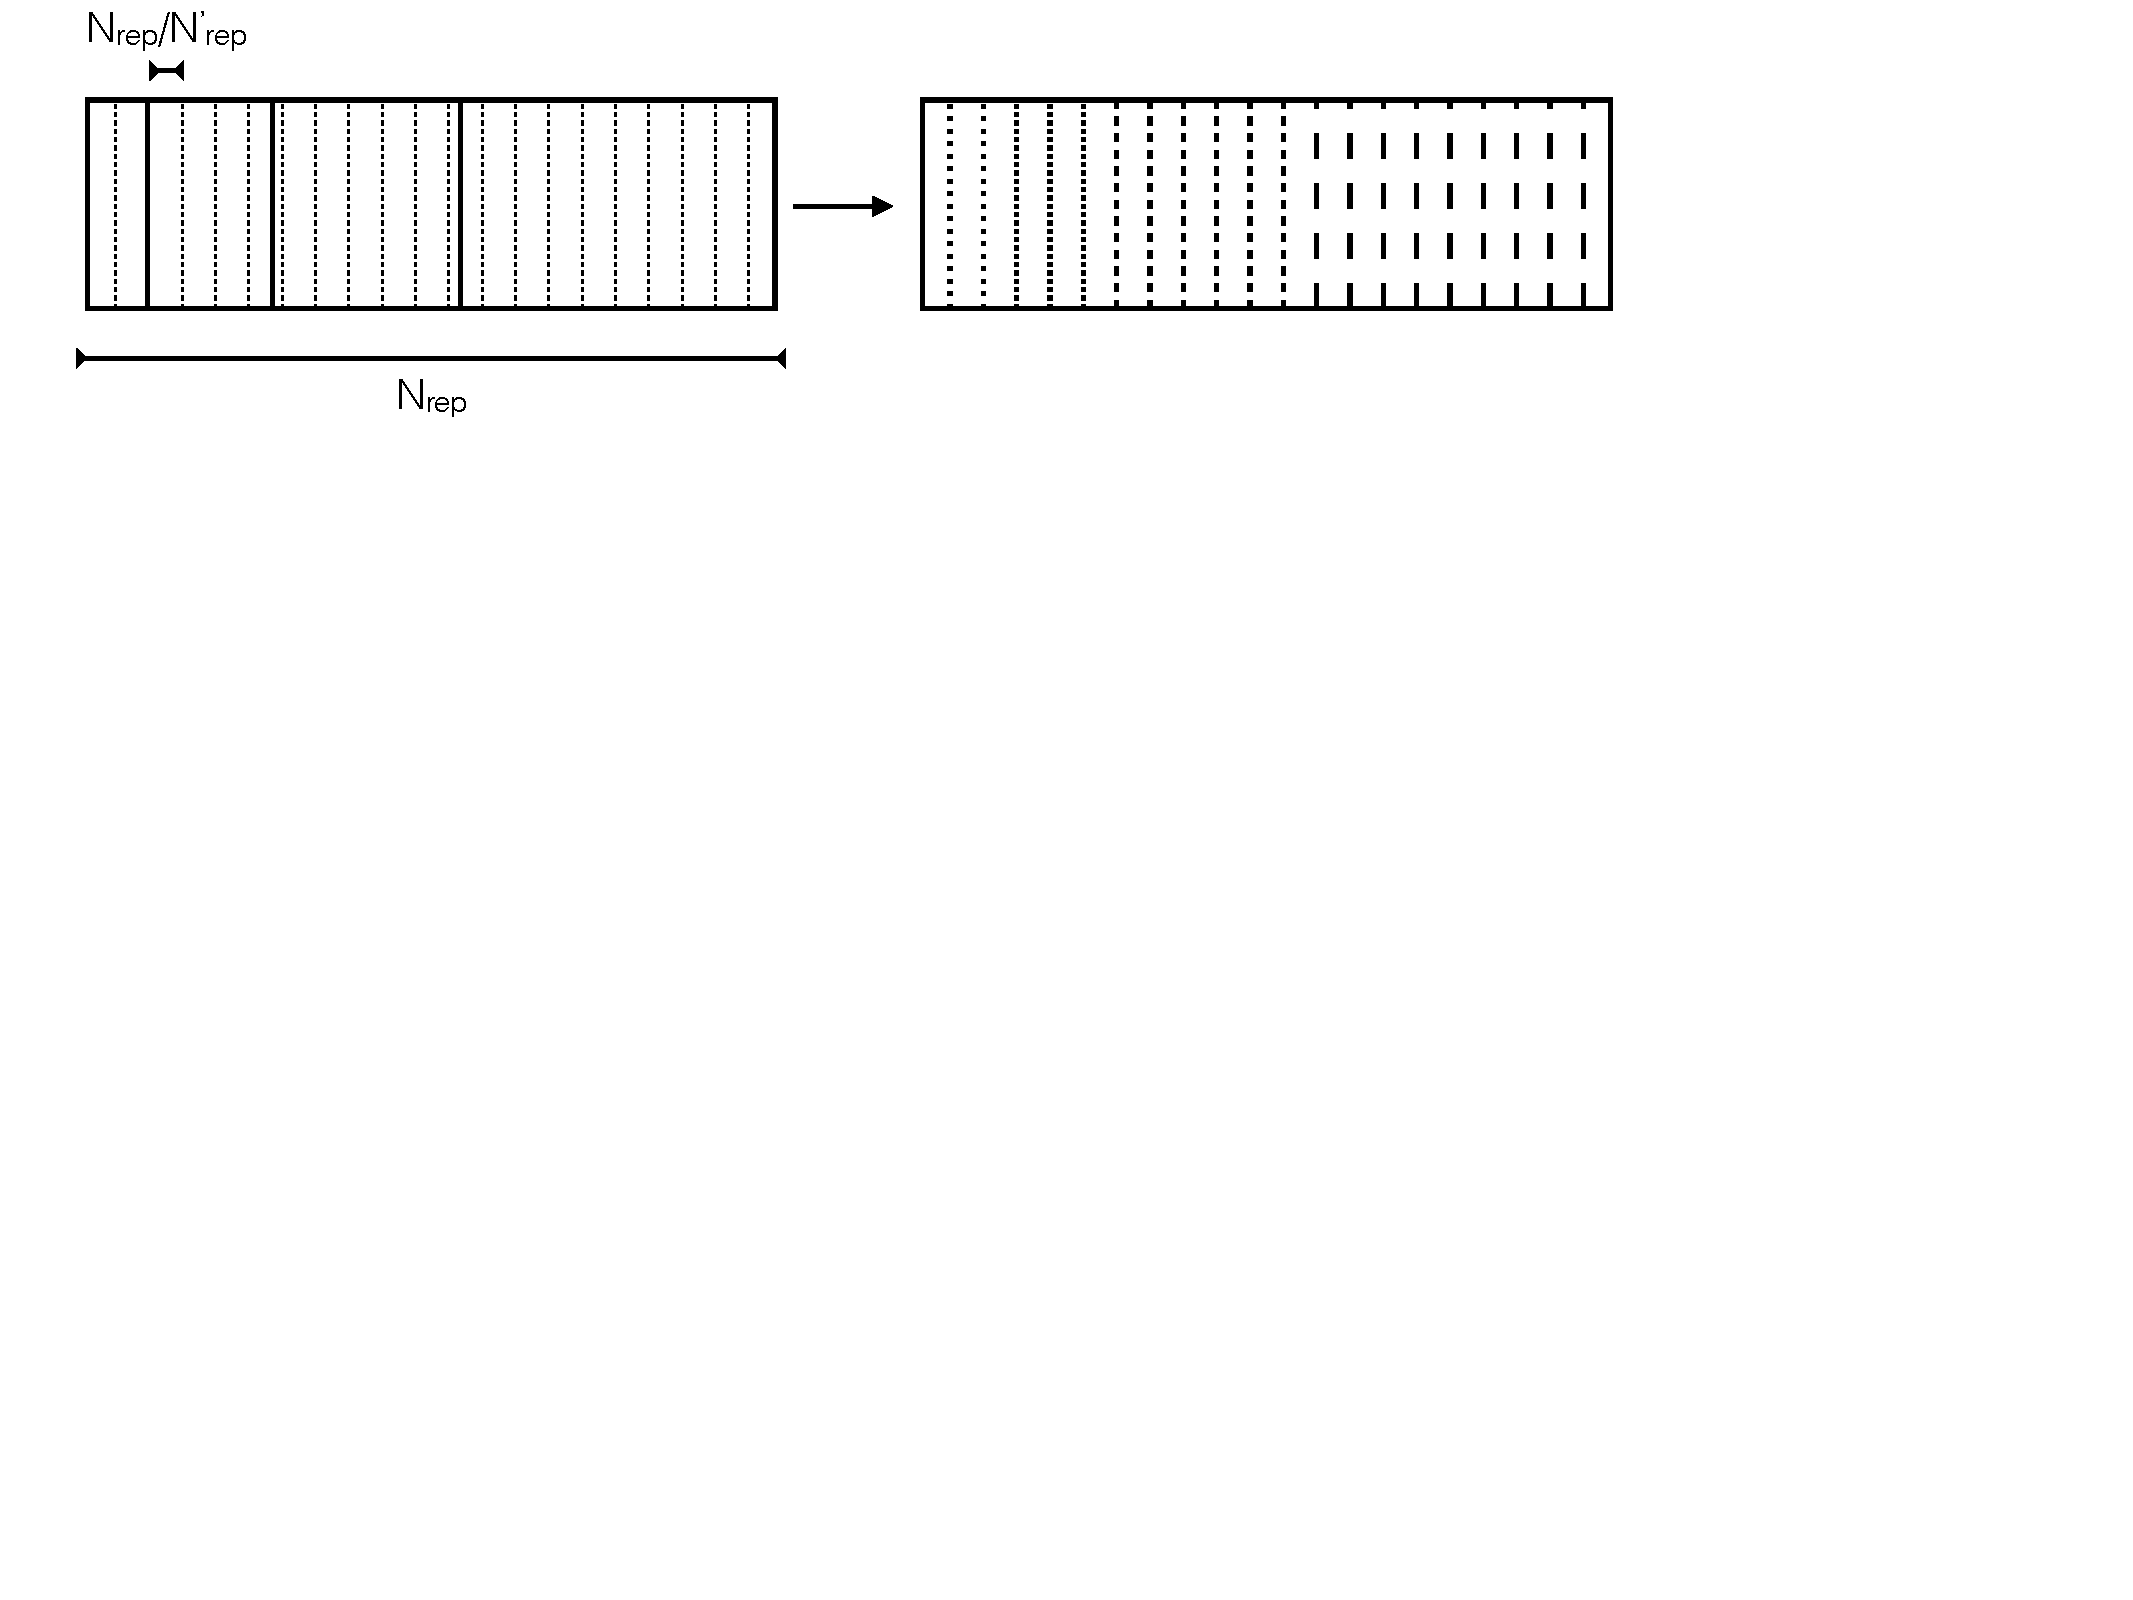
\includegraphics[width=1\textwidth]{4-LHCtools/figs/unweighting.pdf}
\caption[Unweighting of a Bayesian reweighted Monte Carlo PDF set]{The unweighting of a Bayesian reweighted Monte Carlo PDF set. The left hand figure shows the weight cumulant segments for the original weighted set, with four replicas of weight $w_i = \left\{ 1, 2, 3, 4 \right\} $. The line is subdivided by $N_{\text{rep}}^\prime = 20$ lines. The right hand figure illustrates the \emph{unweighted} set in this case. Here each replica in the unweighted set has equal weight, with different line strokes denoting different replicas from the weighted distribution. }
\label{fig:unweighting}
\end{figure}

The weights of the original set are therefore approximately represented as replica multiplicities in the unweighted set, with low-weight replicas selected few times (if at all), and large weight replicas selected multiple times. In this way a conventional MC ensemble can be formed with the usual LHAPDF interface, this time including duplicate replicas for those with high weights and excluding replicas with weights that fall under the unweighted set's resolution. Therefore the unweighting procedure can provide an exact representation of the reweighted ensemble in the limit $N_{\text{rep}}^\prime \to \infty$. 

However in practice a number of unweighted replicas of the order of the number of effective replicas $N_{\text{eff}}$ is typically sufficient for a good level of accuracy in the reproduction.

\subsection{Reweighting validation}
The Bayesian reweighting procedure has been extensively validated by the NNPDF collaboration in a number of highly non-trivial tests of the methodology. As the method has been designed to update a prior distribution with new information analogously to the approach used in an ideal fit, the first test is to ensure that a PDF set reweighted with a new dataset is statistically equivalent to a new set refitted from scratch utilising the new data. This was first performed in~\cite{Ball:2010gb} by reweighting an NNPDF 2.0 fit which included only DIS and Drell-Yan data with information from Tevatron inclusive jet measurements. The reweighted set was compared to the full NNPDF 2.0 fit including the data. As Figure~\ref{fig:rwvalid} demonstrates, the reweighted set is able to reproduce the refitted set up to the level of statistical fluctuation.
\clearpage
\begin{figure}[ht!]
\centering
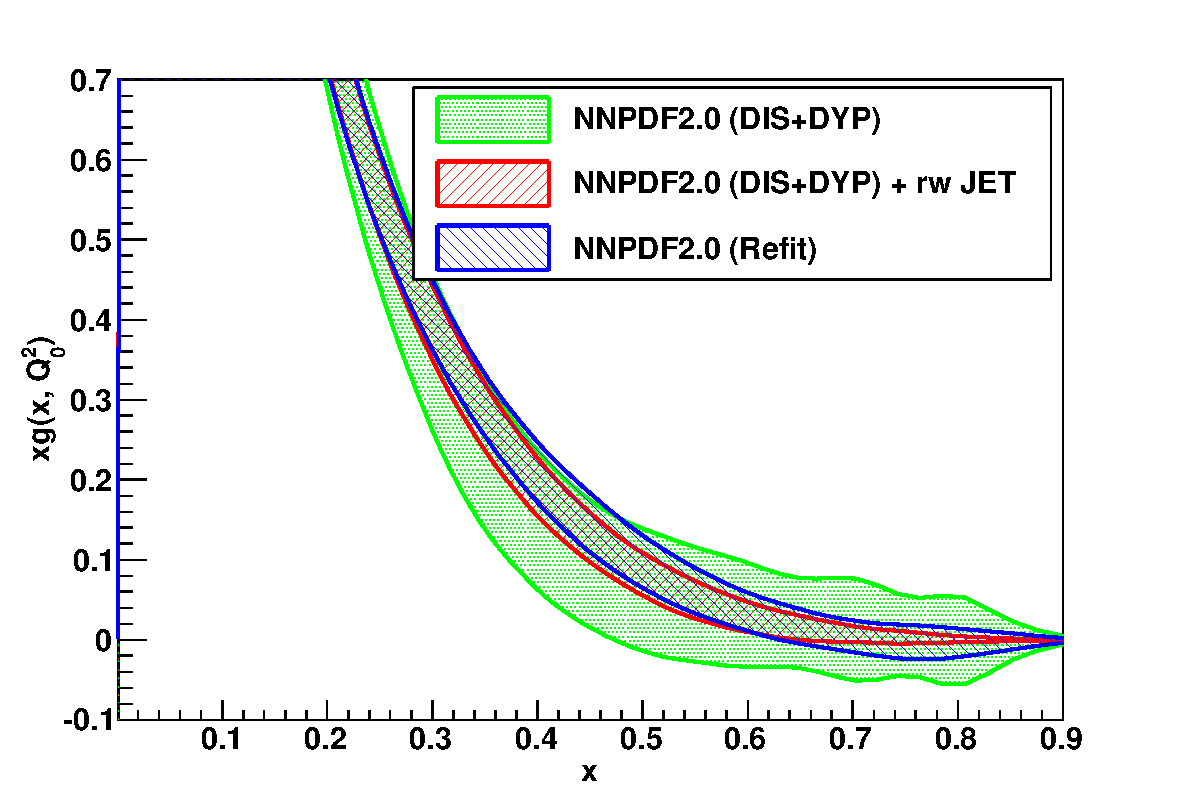
\includegraphics[width=0.45\textwidth]{4-LHCtools/figs/jets-t0-xg_Q2_2_lin.pdf}
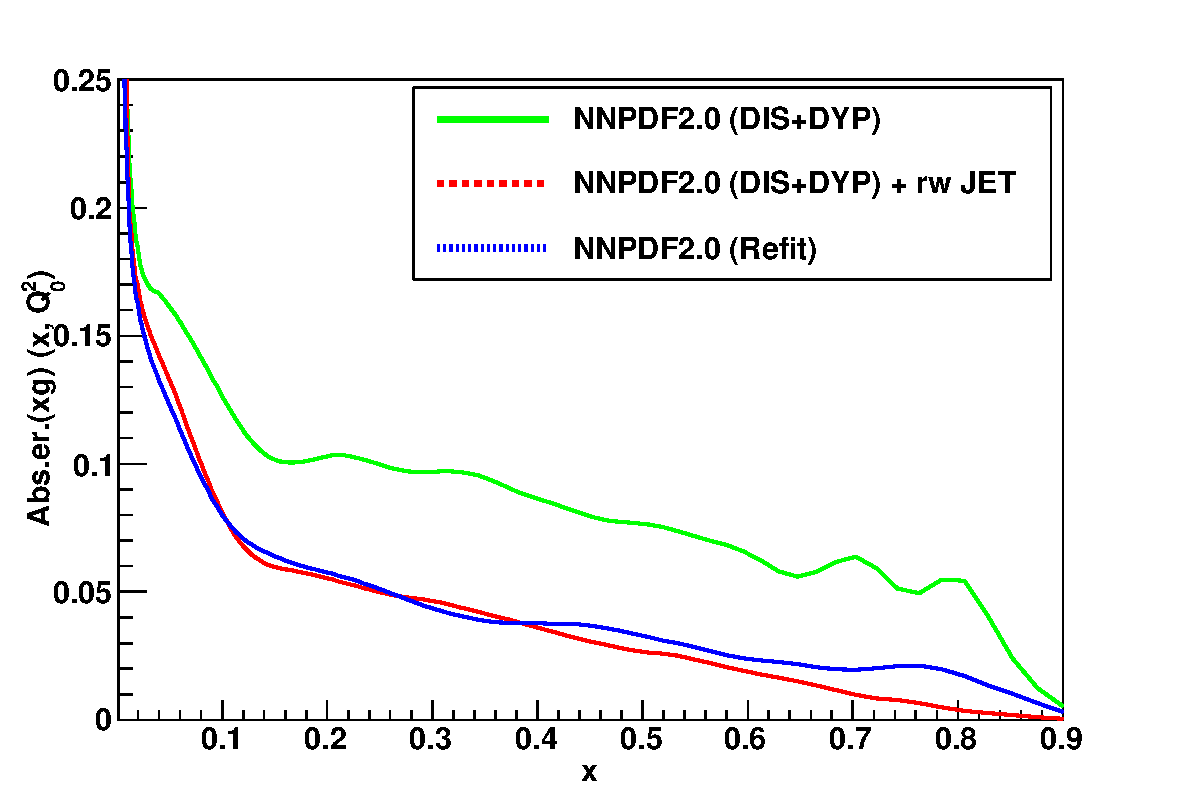
\includegraphics[width=0.45\textwidth]{4-LHCtools/figs/jets-t0-abserror-xg_Q2_2_lin.pdf}
\caption[Validation of Bayesian reweighting by the inclusion of Tevatron jet data]{The validation of Bayesian reweighting by the inclusion of Tevatron jet data. The left figure demonstrates the prior distribution along with the reweighted and refitted distributions upon the addition of Tevatron jet data. The right plot shows the absolute error upon the PDFs for the three sets. Figures are from~\cite{Ball:2010gb}.}
\label{fig:rwvalid}
\end{figure}

The development of the unweighting method as outlined in the previous section, allowed for further tests of the reweighting method. A series of tests were carried out in order to assess the behaviour of PDFs under successive reweighting operations.

When including multiple datasets into a PDF fit via reweighting, there are three possibilities. One can reweight with the combined $\chi^2$ values for the two experiments, or reweight first with one experiment, unweight the PDF ensemble, then reweight with the second. The resulting PDFs should be reasonably independent of the method chosen, and of the order in which the successive reweighting is performed. This requirement is a stringent test of the Monte Carlo PDF representation, as it determines whether or not the ensemble truly behaves as a probability distribution. More pragmatically, the test verifies whether the loss of ensemble efficiency in one reweighting operation is not so great as to prevent a further reweighing. This investigation was carried out in Ref.~\cite{Ball:2011gg} with a DIS only prior. The E605 Drell-Yan experiment and CDF/D0 inclusive jet measurements were included into this set by reweighting. As the E605 experiment provides global fits with rather stringent constraints compared to the moderate effect of the jet data, this is a rather asymmetrical and therefore effective test.



\begin{figure}[ht]
\centering
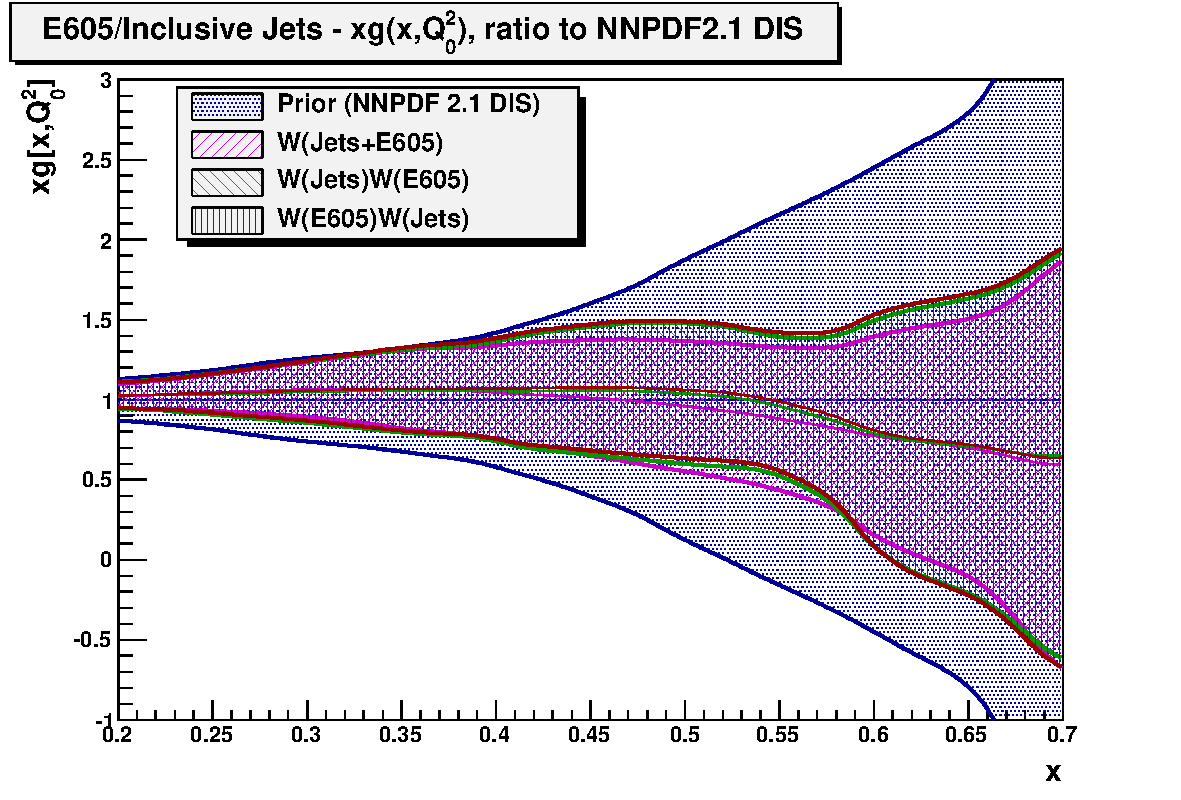
\includegraphics[width=0.48\textwidth]{4-LHCtools/figs/e605-jets_xg_lin_zoom_rel.pdf}
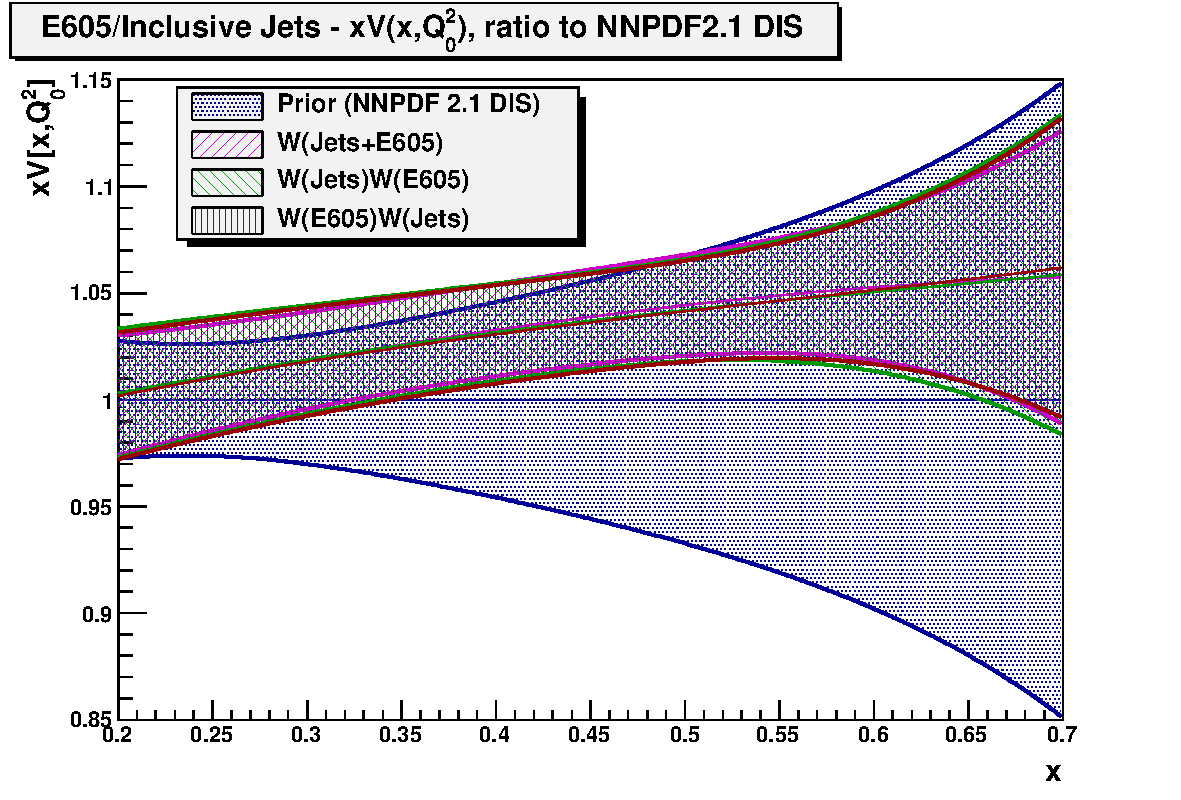
\includegraphics[width=0.48\textwidth]{4-LHCtools/figs/e605-jets_xV_lin_zoom_rel.pdf}
\caption[Test of Bayesian reweighting under a successive reweighting operation]{Test of Bayesian reweighting under a successive reweighting operation. Inclusive Jet and Drell-Yan data are added as a combined dataset, and as individual reweightings separated by an unweighting operation. The resulting distributions, the gluon PDF on the left and the valence distribution on the right, show excellent agreement between the different procedures. All curves are normalised to the prior, NNPDF 2.1 DIS result. The figures are taken from~\cite{Ball:2011gg}.}
\label{fig:SRWvalid}
\end{figure}

In Figure~\ref{fig:SRWvalid} these reweighting procedures are compared for the case of the gluon and valence distributions of the NNPDF2.0 DIS only fit. It is clear that while the impact of the data upon the prior is substantial, the three reweighting methods hardly differ in their results. There is therefore a strong confirmation of the statistical properties of both the Monte Carlo representation of PDFs, and of the reweighting method.

\section{The FastKernel method}
The method of Bayesian reweighting provides an extremely fast and efficient method of including new data into a determination. However as described previously, the method is
ill-suited to the addition of a large or very constraining dataset as the required size of the prior distribution in replicas rapidly becomes unmanageable. Therefore the standard fitting methodology
remains the most important procedure in the determination of parton distributions.

The primary issue in the standard methodology upon the addition of a large LHC dataset is the computational time required to perform the theoretical predictions for experimental data.
Not only must the standard double convolution over the two parton densities be performed, but also each PDF must be evolved from some initial fitting scale to the scale of the experimental data by yet another set of convolutions. We shall first describe the methods used for fast PDF evolution, before going on to discuss the extension to the calculation of physical observables at colliders.

\subsection{Fast PDF evolution}
While there are many methods for performing the evolution of parton distributions, the technique used in NNPDF fits must be particularly efficient due to the computational complexity of the NNPDF procedure. The evolution of a flavour basis PDF of flavour $i$ from an initial scale $Q^2_0$ to a target scale $Q^2_\tau$ can be expressed as 
\be f_i(x_{\alpha}, Q^2_\tau) = \sum_j^{N_{f}} \int_{x_\alpha}^1 d\xi \; \Gamma_{ij}\left(\frac{x_\alpha}{\xi},\frac{Q^2_\tau}{Q_0^2}\right) f_j(\xi, Q_0^2), \label{eq:DGLAPconv} \ee
where the $\Gamma$ are found by solution of the DGLAP equation as shown in Eqn.~\ref{eq:DGLAP}. In order to take advantage of the sparse nature of the DGLAP evolution kernels, we work in the evolution basis defined in Section~\ref{sec:DGLAP},
\be N_i(x_{\alpha}, Q^2_\tau) = \sum_j^{N_{f}} \int_{x_\alpha}^1 d\xi \; \widetilde{\Gamma}_{ij}\left(\frac{x_\alpha}{\xi},\frac{Q^2_\tau}{Q_0^2}\right) N_j(\xi, Q_0^2), \ee
where here we have introduced the notation $N$ for the evolution basis PDFs; related to the flavour basis by a simple rotation
\be f_i(x,Q^2_\tau) =  \sum_j^{N_f}R_{ij}N_j(x,Q_\tau^2). \label{eq:LHA2EVLN}\ee 
Having to perform many instances of the convolution integral in Eqn.~\ref{eq:DGLAPconv} would be prohibitively expensive in most fitting applications, and so an alternative approach must be used. In the NNPDF framework this is based upon the {\tt FastKernel} interpolation method introduced in Ref.~\cite{Ball:2010de}, and shares the general approach with other interpolating methods, while maintaining a hybrid $x$ and Mellin space solution. Here we shall outline the general method used in all interpolating tools.

The first step is to expand the initial-state PDFs upon some set of interpolating basis functions $\mathcal{I}$,
\be f_i(x,Q^2_0) \approx \sum_\beta^{N_{\mathrm{fn}}} c_i^{(\beta)} \;\mathcal{I}^{(\beta)}(x),\ee
with the coefficients of this expansion calculable through the usual overlap integral
\be c^{(\beta)}_i = \int_0^1 dx\;f_i(x,Q^2_0) \; \mathcal{I}^{(\beta)}(x). \ee
Substituting the interpolated version of the initial state PDF into the evolution equation and applying the inverse transformation of Eqn.~\ref{eq:LHA2EVLN} to work in the evolution basis we obtain
\be N_i(x_{\alpha}, Q^2_\tau) = \sum_{j,k}^{N_{f}} \sum_\beta^{N_{\mathrm{fn}}} \int_{x_\alpha}^1 d\xi \; \widetilde{\Gamma}_{ij}\left(\frac{x_\alpha}{\xi},\frac{Q^2_\tau}{Q_0^2}\right) R^{-1}_{jk}\;c_k^{(\beta)} \;\mathcal{I}^{(\beta)}(x). \ee
In this expression, we can actually factorise the PDF-dependent expansion coefficients $c$ from the integral, and perform the convolution over the interpolating functions
\be N_i(x_{\alpha}, Q^2_\tau) = \sum_{k}^{N_{f}} \sum_\beta^{N_{\mathrm{fn}}} E_{ik\alpha\beta}^\tau\;c_k^{(\beta)}, \ee
where the \emph{evolution tables} $E$ are given by 
\be E_{ik\alpha\beta}^\tau =  \sum_{j}^{N_{f}} \int_{x_\alpha}^1 d\xi \; \widetilde{\Gamma}_{ij}\left(\frac{x_\alpha}{\xi},\frac{Q^2_\tau}{Q_0^2}\right) R^{-1}_{jk} \;\mathcal{I}^{(\beta)}(x). \label{eq:evolfactors} \ee
While it may seem as if we have simply moved the problem from the convolution with the DGLAP kernel to the overlap integral required to compute the coefficients $c$, this can be
avoided via a careful choice in the interpolating functions. A suitable choice of interpolating function yields the following identification for the coefficients
\be c_k^{(\beta)} = f_k(x_\beta,Q^2_0),\ee
that is, the interpolants effectively pick out the value of the PDF at some point $\beta$ in an $x$-grid. Providing the grid in $\beta$ is dense enough the interpolation accuracy can still be very high.
With such a choice of functional basis, the full evolution product becomes particularly simple
\ba 
f_i(x_{\alpha},Q^2_\tau) &=&  \sum_{j,k}^{n_f}\sum_{\beta}^{N_x} R_{ij}E^\tau_{\alpha\beta j k}\; f_k(x_\beta,Q^2_0), \\
&=& \sum_{k}^{n_f} \sum_\beta^{N_x} A^\tau_{\alpha\beta ik}\; f_k(x_\beta,Q^2_0). \label{eq:fastPDFfinal}
\ea 
The convolution required by the initial solution to the DGLAP equation has now been reduced via interpolation methods to a simple product over a rotated evolution table $A$.

\subsection{Fast calculation of collider observables}
Similar methods to what we have discussed for fast PDF evolution have also been applied to the calculation of collider observables. For a typical observable with two partons in the initial state,
a full calculation is given by a double convolution over two parton densities,
\be  \sigma_{pp\to X} = \left( \frac{\alpha_s(Q^2)}{2\pi} \right)^{p} \int dx_1\, dx_2\,  f_i(x_1,Q^2)\; d\hat{\sigma}_{ij\to X}\; f_j(x_2,Q^2) \, . \label{eq:hadconv} \ee
The double convolution can once again be avoided by inserting interpolated versions of the PDFs, and performing the convolution over the interpolating functions.
\be  \sigma_{pp\to X} = \left( \frac{\alpha_s(Q^2)}{2\pi} \right)^{p} \sum_{\alpha,\beta}^{N_X}  f_i(x_\alpha,Q^2)\; W_{\alpha\beta,ij}\; f_j(x_\beta,Q^2) \, . \label{eq:hadconv2} \ee
The weight grid $W$ is calculated analogously to the evolution tables in Eqn.~\ref{eq:evolfactors},
\be W_{\alpha\beta,ij} =  \int dx_1\, dx_2\,  \mathcal{I}^{(\alpha)}(x_1)\; d\hat{\sigma}_{ij\to X}\; \mathcal{I}^{(\beta)}(x_2) \, . \ee
Identical methods can be used to interpolate over the hard scale $Q^2$ in multi-scale processes. These techniques are used in publicly available tools such as { \tt APPLgrid}~\cite{Carli:2010rw} and { \tt FastNLO}~\cite{Kluge:2006xs}. In the { \tt APPLgrid} framework, the full product used to calculate a hadronic observable is
\be
\label{eq:applconv}
\sigma = \sum_p \sum_{s}^{N_{\mathrm{sub}}} \sum_{\alpha,\beta}^{N_x} \sum_{\tau}^{N_{Q}}
W_{\alpha\beta\tau}^{(p)(s)} \, \left( \frac{\alpha_s\left(Q^2_{\tau}\right)}{2\pi}\right)^{p}
F^{(s)}\left(x_{\alpha}, x_{\beta},  Q^2_{\tau}\right),
\ee
where the interpolation over a grid of points in hard scale runs over the index $\tau$, and the perturbative order of the contributions is separated by the index $p$. The initial state parton combinations have been grouped into the appropriate QCD subprocesses $s$, according to a table of coefficients $C$,

\be F^{(s)}\left(x_{\alpha}, x_{\beta},  Q^2_{\tau}\right) =  \sum_{i,j}^{13} C^{(s)}_{ij}  \left( f_i(x_{\alpha},Q^2_\tau)f_j(x_{\beta},Q^2_\tau) \right).  \label{eq:APPLsubproc}\ee
The resulting product in Eqn~\ref{eq:applconv} allows for the simple variation of PDFs, strong coupling and perturbative scales in a fast calculation; the product taking typically of order milliseconds rather than the hours to days required to obtain reliable statistics in an NLO code.

Despite the dramatic speed improvement, the { \tt APPLgrid}/{ \tt FastNLO} products represent a considerable computational expense when introducing a large dataset. The NNPDF methodology in particular is extremely sensitive to the convolution speed due to the nature of the genetic algorithm minimisation, orders of magnitude more convolutions are required than in competing approaches. Therefore in order to practically include a large collider dataset into an NNPDF fit more work must be done on improving the convolution algorithm.

\subsection{Combined evolution and observable calculation}
The { \tt APPLgrid}/{ \tt FastNLO} approach maintains a great deal of flexibility, in that scale, $\alpha_S$ and PDF variations are all possible within the same framework. In a PDF fit the only requirement is an efficient variation of input parton distributions. We can therefore try to improve the efficiency of the calculation at the cost of some of the flexibility available in the fast convolution tools. The {\tt FK} procedure and toolchain has therefore been developed, implementing a combined PDF evolution and collider observable calculation.

Recalling the fast PDF evolution method in Eqn.~\ref{eq:fastPDFfinal} with the suitable grids precomputed, PDF evolution can be performed simply as  
\be
f_i(x_{\alpha},Q^2_\tau) = \sum_{k}^{n_f} \sum_\beta^{N_x} A^\tau_{\alpha\beta ik}\; f_k(x_\beta,Q^2_0). \label{eq:fastPDFfinal_recalled}
\ee 
The evolution of the { \tt APPLgrid} subprocess in Eqn.~\ref{eq:APPLsubproc} from an initial state distribution is therefore
\ba F^{(s)}\left(x_{\alpha}, x_{\beta},  Q^2_{\tau}\right) &=&  \sum_{i,j}^{13} \sum_{k,l}^{n_f}  \sum_{\delta,\gamma}^{N_x} C^{(s)}_{ij}  \left[  A^\tau_{\alpha\delta ik}\; f_k(x_\delta,Q^2_0) A^\tau_{\beta\gamma jl}\; f_l(x_\gamma,Q^2_0) \right]\;\;\; \\
&=&   \sum_{k,l}^{n_f}\sum_{\delta,\gamma}^{N_x} \widetilde{C}^{(s),\tau}_{kl,\alpha\beta\gamma\delta} f_k(x_\delta,Q^2_0) f_l(x_\gamma,Q^2_0), \label{eq:FK1}
\ea
where the evolved subprocess coefficients are
\be \widetilde{C}^{(s),\tau}_{kl,\alpha\beta\gamma\delta} = \sum_{i,j}^{13} C^{(s)}_{ij} A^\tau_{\alpha\delta ik} A^\tau_{\beta\gamma jl}.\ee
Substituting the expression for the subprocess in terms of initial state PDFs, Eqn.~\ref{eq:FK1}, into the { \tt APPLgrid} expression for the full convolution shown in Eqn.~\ref{eq:applconv} we obtain
\be
\sigma = \sum_p \sum_{s}^{N_{\mathrm{sub}}} \sum_{\alpha,\beta}^{N_x^\prime} \sum_{\tau}^{N_{Q}}
W_{\alpha\beta\tau}^{(p)(s)} \, \left( \frac{\alpha_s\left(Q^2_{\tau}\right)}{2\pi}\right)^{p}
 \sum_{k,l}^{n_f}\sum_{\delta,\gamma}^{N_x} \widetilde{C}^{(s),\tau}_{kl,\alpha\beta\gamma\delta} f_k(x_\delta,Q^2_0) f_l(x_\gamma,Q^2_0).
\ee
where the number of points in the { \tt APPLgrid} $x$-grid is denoted $N_x^\prime$ to indicate that the grid is different to the input parton $x$-grid which runs over $\gamma,\delta$ up to $N_x$ points. Now that the PDF evolution has been factorised into the coefficients $\widetilde{C}$, much more of this sum may now be precomputed. Specifically we are now able to sum over the indices for subprocess $s$, perturbative order $p$, hard scale $\tau$, and the { \tt APPLgrid} $x-$grids $\alpha$ and $\beta$. The resulting expression for the combined evolution and observable calculation is therefore
\be
\label{eq:FK}
\sigma = \sum_{k,l}^{n_f}\sum_{\delta,\gamma}^{N_x} 
\widetilde{W}_{kl\delta\gamma} \,f_k(x_\delta,Q^2_0) f_l(x_\gamma,Q^2_0),
\ee
with the combined grid, which may be precomputed and stored, given by
\be
\label{eq:FKTable}
\widetilde{W}_{kl\delta\gamma} = \sum_p \sum_{s}^{N_{\mathrm{sub}}} \sum_{\alpha,\beta}^{N_x^\prime} \sum_{\tau}^{N_{Q}}
W_{\alpha\beta\tau}^{(p)(s)} \, \left( \frac{\alpha_s\left(Q^2_{\tau}\right)}{2\pi}\right)^{p}\widetilde{C}^{(s),\tau}_{kl,\alpha\beta\gamma\delta} .
\ee

The quantity $\widetilde{W}_{kl\delta\gamma}$ is the {\tt FK} table for the observable $\sigma$ and encodes all of the theoretical treatment of the observable. The product in Eqn.~\ref{eq:FK} is therefore completely
agnostic with regards to all theory parameters such as process, scales, perturbative order and strong coupling value. This makes the {\tt FK} table particularly simple to implement in a fitting procedure, and allows a clean separation
of theory concerns from the calculation.

The {\tt FK} convolution also benefits from requiring considerably fewer floating point operations than a typical { \tt APPLgrid} convolution. This is particularly evident when studying multi-scale processes, where the sum over the scale grid is precomputed. The product over PDF flavours is now also limited to the $n_f$, typically seven, light partons rather than the general 13 parton basis. Of course in the {\tt FK} procedure the ability to vary scales and the strong coupling with a single grid is lost, and new {\tt FK} tables $\widetilde{W}$ must be generated for different theoretical treatments.

The procedure outlined above for generating {\tt FK} tables from { \tt APPLgrid} or { \tt FastNLO} files has been implemented in a {\tt C++} framework, alongside a comprehensive toolchain for performing {\tt FK} table {\tt I/O} and optimisation. The convolution in Eqn.~\ref{eq:FK} has been implemented for a general PDF input (for example Neural Network or LHAPDF) and extensively optimised. The optimisation ensures only the relevant parton sub channels and $x$-grid entries enter the product, which is performed as a memory-aligned scalar product with the use of SSE intrinsics~\cite{SSE}.   Table~\ref{tab:FKtimings} compares the relative speed improvement compared to the { \tt APPLgrid} calculation of the basic  {\tt FK} convolution and the optimised version, using PDFs obtained through the LHAPDF library.
\begin{table}[htp]
\begin{center}
\begin{tabular}{|c|c|c|c|c|}
\hline Observable &APPLgrid & FK & optimised FK \\
\hline Total $W^+$ xsec &1.03 ms & 0.41 ms (2.5X) & 0.32 ms (3.2X) \\
\hline Jet distribution &2.45 ms & 20.1 $\mu$s (120X) & 6.57 $\mu$s (370X) \\ 
\hline
\end{tabular}
\caption[Comparison of { \tt APPLgrid} and {\tt FK} convolution timings]{Typical timings per observable for several convolution methods. Two observables are presented, the total cross-section for $W^+$ production and the inclusive jet \pt  distribution. Values are given per datapoint. In brackets the relative speed-up compared to the native { \tt APPLgrid} convolution is shown. For this test, the timings were calculated with a 2.9 GHz Intel Core i7 processor.}
\end{center}
\label{tab:FKtimings}
\end{table}
\clearpage
In Table~\ref{tab:FKtimings} a reasonable speed improvement is evident for the example single-scaled process of $W^+$ production, and a very significant improvement on the multi-scale jet production observable. It is important to note that these figures were obtained via convolutions with LHAPDF parton densities, and in a PDF fit a considerably greater speed advantage is gained via the {\tt FK} procedure as no additional operation is required to evolve the PDFs.

While for most applications, the original { \tt APPLgrid} convolution speed is more than sufficient, these speed improvements make the inclusion of a large LHC dataset possible, rather than prohibitively expensive in the NNPDF methodology. For example, in a typical NNPDF fit of 20,000 genetic algorithm generations, including a 100 datapoint jet dataset via the { \tt APPLgrid} interface would add several days of additional computer time to each individual replica fit. With the {\tt FK} procedure this additional cost is reduced to minutes.

The speed improvement is achieved without any loss of accuracy, as the interpolation procedure used to perform the PDF evolution is required in both the { \tt APPLgrid} and {\tt FK} convolutions. The two methods were benchmarked in Ref.~\cite{Ball:2012cx}, with the results shown in Table~\ref{tab:fkbenchatlasjet}. The relative discrepancy $\epsilon$ noted in the table is largely due to the additional interpolation in hard scale $Q^2$ from LHAPDF required in the { \tt APPLgrid} convolution that is not present in the {\tt} FK method, as evolution is performed directly to the required scale.

\begin{table}[ht!]
\begin{center}
\footnotesize
\begin{tabular}{c|c|c|c||c|c|c|}
\cline{2-7}
   & \multicolumn{3}{|c||}{${\rm W}^{+}$ distribution [pb]} & \multicolumn{3}{|c|}{${\rm W}^{-}$ distribution [pb]}  \\
\hline
\multicolumn{1}{|c||}{$| \eta_{l} |$} & {\tt FK}	 & {\tt APPLgrid} &  $\epsilon_{\rm rel}$ & {\tt FK}  &  {\tt APPLgrid} &  $\epsilon_{\rm rel}$\\
\hline
\multicolumn{1}{|c||}{0.00--0.21} & 617.287 & 617.345 & 0.01\% & 456.540 & 456.819 & 0.06\% \\
\multicolumn{1}{|c||}{0.21--0.42} & 616.988 & 617.062 & 0.01\% & 453.045 & 453.315 & 0.06\%\\
\multicolumn{1}{|c||}{0.42--0.63} & 620.237 & 620.290 & 0.01\% & 448.902 & 449.172 & 0.06\%\\
\multicolumn{1}{|c||}{0.63--0.84} & 624.192 & 624.235 & 0.01\% & 441.789 & 442.045 & 0.06\%\\
\multicolumn{1}{|c||}{0.84--1.05} & 630.235 & 630.286 & 0.01\% & 432.206 & 432.435 & 0.05\%\\
\multicolumn{1}{|c||}{1.05--1.37} & 636.835 & 636.886 & 0.01\% & 419.027 & 419.222 & 0.05\%\\
\multicolumn{1}{|c||}{1.37--1.52} & 642.800 & 642.861 & 0.01\% & 403.908 & 404.084 & 0.04\%\\
\multicolumn{1}{|c||}{1.52--1.74} & 642.499 & 642.569 & 0.01\% & 390.564 & 390.724 & 0.04\%\\
\multicolumn{1}{|c||}{1.74--1.95} & 642.351 & 642.437 & 0.01\% & 377.328 & 377.473 & 0.04\%\\ 
\multicolumn{1}{|c||}{1.95--2.18} & 628.592 & 628.693 & 0.02\% & 359.373 & 359.498 & 0.03\%\\
\multicolumn{1}{|c||}{2.18--2.50} & 590.961 & 591.079 & 0.02\% & 337.255 & 337.366 & 0.03\% \\
\hline
 \end{tabular}
 
 \vspace{2mm}
 
 \begin{tabular}{c|c|c|c|}
 \cline{2-4}
   & \multicolumn{3}{|c|}{Z distribution [pb]}  \\
    \hline
\multicolumn{1}{|c||}{$|y|$} & {\tt FK}	  &    {\tt APPLgrid}  &   $\epsilon_{\rm rel}$\\
\hline
\multicolumn{1}{|c||}{0.0--0.4} & 124.634 & 124.633 & 0.001\%\\
\multicolumn{1}{|c||}{0.4--0.8} & 123.478 & 123.488 & 0.01\%\\
\multicolumn{1}{|c||}{0.8--1.2} & 121.079 & 121.108 & 0.02\%\\
\multicolumn{1}{|c||}{1.2--1.6} & 118.057 & 118.108 & 0.04\%\\
\multicolumn{1}{|c||}{1.6--2.0} & 113.512 & 113.549 & 0.03\%\\
\multicolumn{1}{|c||}{2.0--2.4} & 106.552 & 106.562 & 0.01\%\\
\multicolumn{1}{|c||}{2.4--2.8} & 93.7637 & 937.838 & 0.02\%\\
\multicolumn{1}{|c||}{2.8--3.6} & 55.8421 & 558.538 & 0.02\%\\
\hline
 \end{tabular}
 
  \vspace{2mm}
  
\begin{tabular}{c|c|c|c|}
\cline{2-4}
   & \multicolumn{3}{|c|}{ATLAS 2010 jets [pb]}  \\
    \hline
\multicolumn{1}{|c||}{$p_T$ (GeV)} & {\tt FK}	  &    {\tt APPLgrid}  &    $\epsilon_{\rm rel}$ \\
\hline
\multicolumn{1}{|c||}{20--30}   & $6.1078 \times 10^6$ & $6.1090 \times 10^6$ &	0.02\% \\
\multicolumn{1}{|c||}{30--45}   & 986285 	                     & 98654      & 0.03\% \\
\multicolumn{1}{|c||}{45--60}   & 190487 	                     & 190556    & 0.04\% \\
\multicolumn{1}{|c||}{60--80}   & 48008.7 	                     & 48029.7   & 0.04\% \\
\multicolumn{1}{|c||}{80--110} & 10706.6 	                     & 10710.4   & 0.03\% \\
\multicolumn{1}{|c||}{110--160} & 1822.62 			  & 1822.87   & 0.01\% \\
\multicolumn{1}{|c||}{160--210} & 303.34 			  & 303.443   & 0.03\% \\
\multicolumn{1}{|c||}{210--260} & 76.1127 			  & 76.1338   & 0.03\% \\
\hline
 \end{tabular}

 \end{center}
\caption[Benchmark of the {\tt FK} result for datasets with different underlying processes]{ Benchmark of the {\tt FK} result for datasets with different underlying processes, all generated according to ATLAS experimental kinematics and acceptances. The { \tt APPLgrid} and {\tt FK} results are presented along with the relative discrepancy between the two. Table from \cite{Ball:2012cx}.\label{tab:fkbenchatlasjet} }
\end{table}
%%%%%%%%%%%%%%%%%%%


%

%
%\be f_i(x_{\alpha},Q^2_\tau) =  \sum_j^{13}R_{ij}N_j(x_{\alpha},Q_\tau^2) =\sum_{j}^{13} \sum_{\gamma}^{N_x}  \sum_{k}^{N_{\mathrm{pdf}}} R_{ij}E^\tau_{\alpha\gamma j k}N^0_k(x_\gamma).\ee 
%\be F^{(l)}\left(x_{\alpha}, x_{\beta},  Q^2_{\tau}\right) =   \sum_{i,j}^{13} \sum_{k,l}^{N_{\mathrm{pdf}}}  C^{(l)}_{ij}A^\tau_{\alpha\gamma i k}A^\tau_{\beta\delta j l}N^0_k(x_\gamma)N^0_l(x_\delta),
%\quad\quad A^\tau_{\alpha\gamma i k} =  \sum_j^{13} R_{ij}E^\tau_{\alpha\gamma j k}.\ee
%\be \sigma =  \sum_{i,j}^{N_{\mathrm{pdf}}} \sum_{\alpha,\beta}^{N_x} \widetilde{W}_{\alpha\beta i j} N_i^0(x_\alpha)N_j^0(x_\beta),\ee
%\be \widetilde{W}_{\alpha\beta i j} = \sum_p \sum_{l=0}^{N_{\mathrm{sub}}}\sum_{k,l}^{13} \sum_{\gamma,\delta}^{N_x} \sum_{\tau}^{N_{Q}}
%W_{\gamma\delta\tau}^{(p)(l)} \, \left( \frac{\alpha_s\left(Q^2_{\tau}\right)}{2\pi}\right)^{p} C^{(l)}_{kl}A^\tau_{\gamma\alpha k i}A^\tau_{\delta\beta l j}, \ee
%

\section{Interpolating tools for automated NLO}
Tools such as { \tt FastNLO}/{ \tt APPLgrid} and their extension for fast PDF fitting in the $\tt FK$ method, are invaluable in the analysis of collider data. Their usefulness is not limited to applications such as fitting, but can also be used to perform thorough QCD analysis with rigorous theory uncertainty estimation in situations where obtaining sufficient statistics with an NLO code or event generator would be extremely expensive computationally. Despite this, at the outset of LHC data taking the amount of codes interfaced to such interpolating tools was extremely limited. Additionally the need for separate interfaces to existing codes meant a great deal of duplication in terms of analysis tools and software.  The { \tt APPLgrid} group provided a direct interface to the NLO codes {\tt MCFM}~\cite{Campbell:2000bg} and {\tt nlojet++}~\cite{Nagy:2001fj,Nagy:2003tz}. { \tt FastNLO} provided a set of precomputed scenarios generated through a private interface to NLO codes. More recently, a public toolkit was released to allow for the interfacing of { \tt FastNLO} to external calculations. 

A conspicuous absence was an interface to tools providing automated NLO calculations via computer algebra suitable one-loop methods\cite{Anastasiou:2006jv,Berger:2008sj,Denner:2005nn,Ellis:2007br,Giele:2008ve,Ossola:2006us} and their implementations in parton level Monte Carlo codes such as {\tt MadGraph}~\cite{Alwall:2011uj}, {\tt HELAC}~\cite{Bevilacqua:2011xh} and {\tt SHERPA}~\cite{Gleisberg:2003xi,Gleisberg:2008ta}. In this section we shall discuss the implementation of a fast interface to such codes, the {\tt MCgrid}~\cite{DelDebbio:2013kxa} package; developed with the aid of funding from the MCnet initial training network.  


\subsection{Reweighting Monte Carlo calculations}
Recalling Eqn.~\ref{eq:hadconv}, a hadronic observable calculation proceeds via
\be  \sigma_{pp\to X} = \sum_p \left( \frac{\alpha_s(Q^2)}{2\pi} \right)^{p} \int dx_1\, dx_2\,  F_l(x_1,x_2,Q^2)\; d\hat{\sigma}_{l\to X}^{(p)}\; , \label{eq:doubleconv2} \ee
where the initial state PDFs have been grouped according to Eqn.~\ref{eq:APPLsubproc} and the sum over subprocesses is implicit. In an event generator this integral is performed via Monte Carlo integration. At leading order this is a relatively straightforward procedure,
\begin{align}
  \label{eq:basicMC}
  \sigma_{pp\to X}^{\text{LO}} &= \sum_{e=1} \tilde{w}_e(k_e) = \sum_{e=1}^{N_\evt} \left(  \frac{\alpha_s\left(k_e\right)}{2\pi} \right)^{p_{\text{LO}}} w_e(k_e) F_{l_e}(k_e)\, ,
\end{align}
where $\tilde{w}$ is the full event weight and the $w$ are the matrix element weights generated via importance sampling of the integrand of Eqn.~\ref{eq:doubleconv2}. The $F_{l_e}$ refer to the parton density of the event's subprocess $l_e$. Each event is generated according to a set of kinematics
\begin{align}
  k_e &= \left\{p_1, ..., p_n,\,x_1,\,x_2,\,\frac{\mu_F^2}{Q^2},\,\frac{\mu_R^2}{Q^2} \right\}.
\end{align}

As a full re-run of the event generator for every parameter variation is extremely expensive, the variation is typically performed via an event-by-event reweighting procedure. The full set of events is stored
in a common format such as { \tt HepMC}~\cite{Dobbs:2001ck} and re-processed by dividing out the appropriate factors of the old PDFs and $\alpha_S$ and multiplying in the desired new values. 

\be \tilde{w}_e (k_e)\to \left(  \frac{\alpha_s^\prime\left(k_e\right)}{\alpha_s\left(k_e\right) } \right)^{p_{\text{LO}}}  \frac{F^\prime_{l_e}(k_e)}{F_{l_e}(k_e)}\; \tilde{w}_e(k_e), \ee
where the primed quantities denote the new, reweighted strong coupling and PDF choices. Having the full generated event sample stored also has the advantage of being able to rerun analysis software with varying parameters/selections without the need to rerun the potentially expensive event generation.

The reweighting situation in an NLO calculation is considerably more complicated. In order to be able to solve the integral numerically, a divergence-subtraction scheme e.g Catani-Seymour~\cite{Catani:1996vz}
or Frixione-Kunst-Signer (FKS)~\cite{Frixione:1995ms,Frixione:1997np} must be employed. These subtraction algorithms separate the calculation into distinct sections which are to be numerically evaluated individually. Here we shall discuss the implementation in terms of a Catani-Seymour dipole scheme. The four contributions to the total NLO cross section are 

\begin{equation}
  \label{eq:NLOxsect}
  \sigma_{pp\to X}^{\text{NLO}}= \int d\hat{\sigma}^\mathrm{B}
  + \int d\hat{\sigma}^\mathrm{V}
  + \int d\hat{\sigma}^\mathrm{I}
  + \int d\hat{\sigma}^\mathrm{RS}
  \, .
\end{equation}
The terms $B$, $V$, $I$ and $RS$ refer to the Born (B), Virtual (V), Integrated subtraction (I) and Real Subtracted (RS) cross section elements respectively. Neglecting terms used in the variation of perturbative scales, the $B$, $V$ and $RS$ terms may be integrated via a Monte Carlo procedure equivalently to Eqn.~\ref{eq:basicMC}. The integrated dipole term however has a rather more complicated dependance upon the initial state PDFs, originating as it does through the splitting of an initial state parton. The Monte Carlo solution to the $I$ integral is given by 

\def\varref#1{{\tt #1}}
\begin{eqnarray}
 \int d\hat{\sigma}^\mathrm{I}  &=&  \sum_{e=1}^{N_\evt}   \left(  \frac{\alpha_s(\mu_R^2)}{2\pi} \right)^{p_{\text{NLO}}} \Bigg\{  F_{l_e}(x_1,x_2,\mu^2_F)\,  w^{(0)}_e 
\nonumber\\
&&+\sum_{s}^{N_{\text{sub}}} F_s(x_1/x'_1, x_2, \mu^2_F)\, \tilde{w}^{(1)}_{e,s} \label{eq:NTupleBreakdown} \\
&&+\sum_{s}^{N_{\text{sub}}} F_s(x_1, x_2/x'_2, \mu^2_F)\, \tilde{w}^{(2)}_{e,s}
 \Bigg\},
  \, \nonumber 
\end{eqnarray}
in which the weight $w^{(0)}$ arises through the usual Born-like PDF dependance, and the weights $w^{(1/2)}$ arise from integration over parton-$x$ from the first or second parton in the initial state splitting. To reweight such events these weights must therefore be properly distinguished
in the event record. While is is not the case in the standard {\tt HepMC} layout, a format based upon {\tt ROOT NTuples} was designed by the {\tt BlackHat-Sherpa} group for the reweighting of NLO event weights~\cite{Bern:2013zja}. In the {\tt BlackHat NTuple} format the weights that must be distinguished for the accurate treatment of scale variations are also stored.  \\
While the event reweighting approach is considerably faster than an entire rerun of the Monte Carlo, a reweight of a full event sample can still take a considerable amount of computer time. The key issue being that the statistical accuracy of the calculation is limited by the number of events in the sample, and therefore for a more accurate calculation, more computational expense is incurred. This dependence on the event loop is not removed by the event reweighting procedure. The dependance can however be removed by applying the interpolation methods of the previous section, by providing an interface for event generators to interpolating packages such as { \tt APPLgrid}.
\subsection{An interpolation interface for automated NLO} 
\label{sec:interp}
The {\tt MCgrid} project began as a direct interface for the {\tt SHERPA} event generator framework to the {\tt APPLgrid} interpolation package. The development of a new interface between an event generator and the {\tt APPLgrid} framework in principle requires the implementation of an analysis suite to provide the categorisation of event final states into appropriate observable bins. However the {\tt MCgrid} interface is built upon standard analysis tools and formats to provide a more general interface between standards-compliant Catani-Seymour event generators to the {\tt APPLgrid} package.

{\tt MCgrid} is written as a set of additional tools for the {\tt Rivet} MC analysis system. The {\tt Rivet} system implements a wide range of experimental analysis tools and provides the flexibility for the user to define their own selection criteria and processing tools to operate on an event final state. Writing the {\tt APPLgrid} interface as a {\tt Rivet} extension therefore removes the need to implement a separate toolchain, and allows a degree of generator agnosticism. As {\tt} Rivet operated upon events in the standard {\tt HepMC} format, any generator equipped to output events in this format may potentially be interfaced to {\tt APPLgrid} through {\tt MCgrid}.

The interface requires additional information over the standard data available in {\tt HepMC}, as the information on the weight breakdown as per Eqn.~\ref{eq:NTupleBreakdown} must be available. However this can be straightforwardly appended in the {\tt HepMC} user defined weights fields. The interface then provides the correct handling of initial state parton mappings from the PDF basis used in the Catani-Seymour process to the APPLgrid flavour basis.

With the appropriate mapping to initial state parton flavours performed, the weights must be converted to the appropriate subprocess basis. The minimal initial state PDF basis can be automatically determined by a set of packaged scripts.
General purpose Monte Carlo codes such as {\tt SHERPA} will typically generate events will the full initial parton flavours explicit rather then generating events based upon QCD subprocesses. Weights originating from different flavour basis channels are generated via importance sampling of the distribution in order to ensure an efficient description of the most important channels.  Accordingly there is a selection weight present in each event weight, given by 
\begin{equation}  
w_e(i,j,k_e) =\mathcal{N}_{ij}\;d \hat{\sigma}_{l_e \to X}(k_e) \Pi_{\text{ps}}(k_e) \Theta (k_e-k_{\text{cuts}}), \label{eq:mcweight}
\end{equation}
where the factor $\mathcal{N}_{ij}$ is approximately given by
\begin{equation}
\mathcal{N}_{ij} \sim \frac{N_{\text{tot}}}{N_{ij}}, \label{eq:selectionweight}
\end{equation}
where $N_{\text{tot}}$ denotes the total number of events in the sample, and $N_{ij}$ is the number of events initiated by partons of flavour $i$ and $j$. In Eqn.~\ref{eq:mcweight} we use $\Pi$ to represent the phase space weight associated with the kinematics $k_e$, and the $\Theta$ as a step function implementing the desired kinematic cuts in the analysis. 
The selection weights $\mathcal{N}$ must be converted into the appropriate subprocess selection weight to prevent the statistical uncertainty in poorly-sampled distributions from overwhelming the subprocess. {\tt MCgrid} monitors the relative population of the channels and subprocesses in order to provide a statistically sound subprocess combination. The selection weight in Eqn.~\ref{eq:selectionweight} must be converted into the appropriate subprocess selection weight as
\be \mathcal{N}_{ij} \to \mathcal{N}_{l} = \frac{N_{\mathrm{tot}}}{N_{l}}, \ee
where $N_{l}$ is the number of events falling into the initial state subprocess $l$. Converting the selection weights to the appropriate subprocess selection weight is therefore a matter of multiplying each event weight by a factor $N_{ij}/N_{l}$.


In this way the fully exclusive predictions given in a typical Monte Carlo event generator may be effectively converted into the relevant subprocess basis. With this accomplished, and the correct weight conversion performed according to the exact PDF dependance of the Catani-Seymour counterterms, the weights may be filled directly into an APPLgrid type weight grid. Figure~\ref{fig:MCgridreps} demonstrates the application of the {\tt MCgrid} package when used in conjunction with {\tt Sherpa} and {\tt BlackHat} as a one-loop generator. The tools are applied to the test cases of Drell-Yan and inclusive jet production, with the resulting { \tt APPLgrid} applied to the estimation of scale and $\alpha_S$ uncertainties alongside standard PDF error, requiring a very large number of replicas.

The {\tt MCgrid} project is publicly available\footnote{The software is available at \emph{http://mcgrid.hepforge.org}.}, and allows for the first time calculations from automated NLO event generators to be interfaced to interpolation tools, for potential application in PDF fits, or indeed fast parameter variation studies in phenomenological applications.

\begin{figure}[h!]
\centering
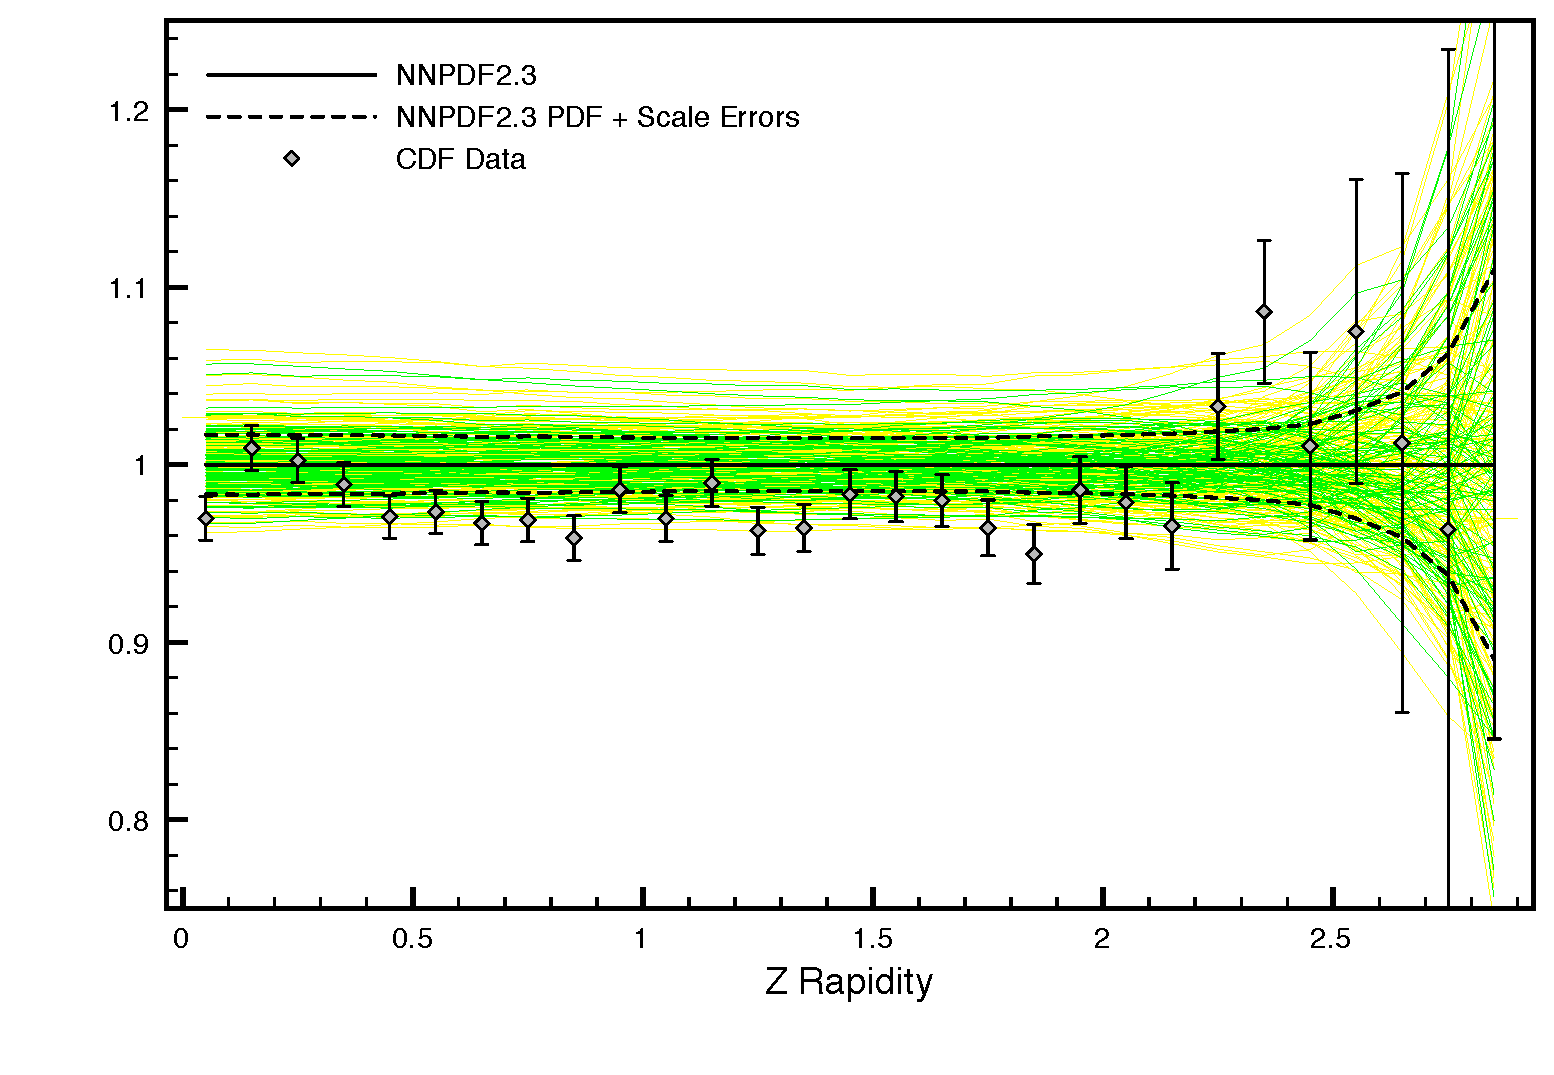
\includegraphics[width=0.48\textwidth]{4-LHCtools/figs/100MDYReplicas_Scales.pdf}
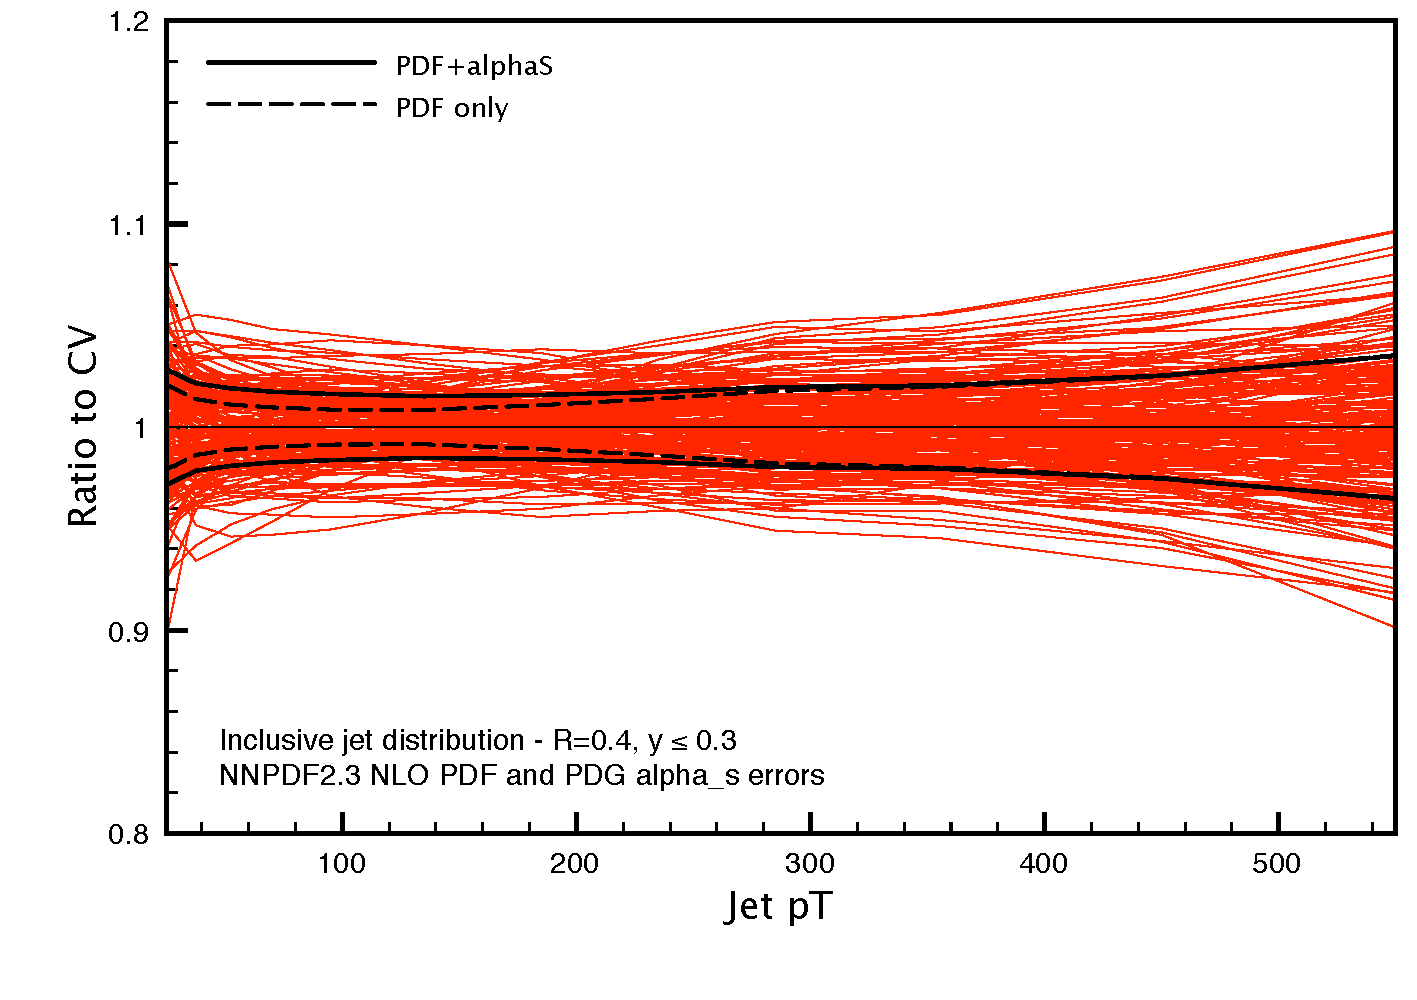
\includegraphics[width=0.48\textwidth]{4-LHCtools/figs/JetsAlphas_0.pdf}
\caption[An example of the output of the {\tt MCgrid} package]{An example of the output of the {\tt MCgrid} package. A $Z$ boson rapidity distribution plot is shown on the left, with scale error estimation. The plot on the right demonstrates the grids applied to inclusive jet data, with $\alpha_S$ error estimation. Both plots are normalised to their central values, to demonstrate the level of uncertainty.}
\label{fig:MCgridreps}
\end{figure}